% chktex-file 1   user-defined macros (\NumPrimes etc.) terminated with space is correct
% chktex-file 8   en-dash compounds are correct academic usage
% chktex-file 12  interword spacing in captions is intentional
% chktex-file 13  intersentence spacing is a style choice
% chktex-file 18  \MakeOuterQuote{"} is active in report_main.tex
% chktex-file 24  \label on own line is standard practice
\chapter{Constructing the DoD Semiconductor Supply Chain}
\label{chap:dod-supply-chain}

Supply-chain visibility in commercial data is fundamentally incomplete: many real supplier--customer relationships are simply undisclosed. This report treats incompleteness as a predictive problem on FactSet Supply Chain Relationships (SCR), framed as positive--unlabeled link prediction, where measured precision serves as a conservative lower bound. Building on that framing, Section~\ref{chap:link-prediction} establishes a calibrated ensemble ranking. It defines explicit selection policies---most importantly, per-source Top-K style operating rules---that yield a high-precision set of inferred links suitable for downstream use. Section~\ref{chap:dod-supply-chain} shifts from prediction to construction. Rather than treating the global SCR graph as the object of analysis, the analysis uses the ranked and policy-filtered outputs as controlled inputs to build a DoD-anchored semiconductor network, in which the central empirical task is to make defense-relevant dependencies visible in a way that supports risk analysis, because, in this domain, visibility precedes defense.

The construction assembles the DoD-anchored semiconductor subgraph by merging complementary evidence streams that, on their own, each provide only partial visibility into multi-tier dependence. The build treats DoD demand as Tier-0---operationalized not as a single "DoD" super-node, but as the specific awarding components through which procurement is executed (for example, the Department of the Army, Department of the Navy, Department of the Air Force, the Defense Logistics Agency (DLA), and the Defense Information Systems Agency (DISA)). From these component-level demand nodes, Tier-1 is defined as the set of prime vendors that receive direct DoD contract obligations within a fixed window. The construction then expands outward from these seeds using three relationship layers: disclosed supplier--customer links from FactSet SCR, observed connectivity from shipping transactions, and a high-confidence subset of predicted edges selected using the calibrated ensemble ranking and operating policies established earlier. Lower tiers enter only through these disclosed, observed, and predicted layers introduced in subsequent subsections. The resulting network is sparse and directed, anchored in procurement reality while extending beyond what any single data source can reveal, and it provides the empirical foundation for the structural analyses in Section~\ref{chap:network_analysis}.

The section proceeds in a sequence that mirrors the construction problem. It begins by using USAspending.gov to define DoD component demand nodes and prime-vendor recipients. Then it maps those contracting identifiers into the commercial entity framework required to connect the seed set to FactSet. Relationship evidence is then incorporated in layers---disclosed SCR ties, shipping-based connections, and high-confidence predicted links selected under the operating policies established earlier---and consolidates them into a single directed network representation. After integration, the network is pruned to a semiconductor-relevant subgraph and summary diagnostics are presented that describe how each evidence layer contributes to coverage and structure. To keep the build reproducible and leakage-safe, the build constructs the network as a point-in-time snapshot, governed by a fixed-point-in-time build (2025-06-09) that aligns contracting, disclosed, shipping, and model-based inputs. Throughout, edges are treated as evidence of a relationship under a defined source---contracting tie, disclosed supplier--customer link, shipment connection, or high-confidence predicted relationship---rather than item-level provenance tracing a specific chip into a specific platform. The section closes by specifying the limits of visibility that remain even after layering---in particular the absence of systematic subcontractor and lower-tier disclosure in contracting data---and by explaining how those limits condition the interpretation of subsequent results.

%========================
% Section 3.1
%========================
\section{Tier-0 and Tier-1 Construction}

The demand anchor draws on federal contracting to define the network in observed DoD demand. Specifically, Tier-0 and Tier-1 are drawn from USAspending.gov, which reports federal award transactions under the standardized disclosure regime established by the Digital Accountability and Transparency Act of 2014 \parencite{us_congress_digital_2014}. Tier-0 is the set of DoD awarding components---treated as distinct demand nodes rather than collapsed into a single "DoD" super-node---and Tier-1 is the set of prime recipients that receive direct DoD contract obligations within the analysis window \parencite{us_department_of_the_treasury_data_2025}. From these records, the construction produces a deduplicated seed edge list linking each awarding component to each prime recipient it directly obligates. The matching step then maps those primes to the FactSet entity universe, enabling the government data to connect to the commercial relationship layers introduced in subsequent subsections.

Tier-0 and Tier-1 are defined operationally at the level of identifiers available in the transaction-grain contracting data. For Tier-0, the awarding organization serves as the relevant DoD ``demand node''. It implements this at the component or sub-agency level, rather than aggregating all procurement into a single DoD entry point. Preserving meaningful heterogeneity in how procurement is executed across the Department---for example, between the military departments and defense agencies---ensures that the first layer of the network reflects the actual institutional channels through which obligations are made. For Tier-1, primes are defined as the recipients recorded on DoD contract transactions in USAspending during the study window, recognizing that these recipients are the entities legally responsible for contract performance at the prime level in the federal reporting system. These tier definitions are strictly local to the demand-anchor stage: they identify who obligates and who is obligated in direct contracting records, while leaving any claims about subcontracting or lower-tier production dependencies to the relationship layers that follow.

To keep construction reproducible and align contracting with the other evidence streams used later in this section, the demand anchor is built as a point-in-time snapshot, governed by a fixed-point-in-time build dated 2025-06-09. The Tier-0/Tier-1 seed set is defined for FY2022--FY2025 using USAspending as of that date, limiting inclusion to information observable at the snapshot time and reducing the risk of incorporating later revisions. This section selects FY2022--FY2025 because it provides a recent, policy-relevant picture of DoD procurement while spanning enough fiscal years to smooth idiosyncratic timing effects in contracting and produce a stable set of prime recipients. Holding the window fixed also standardizes the denominator for the coverage and attrition statistics reported later in this section.

The pipeline ingests DoD award transaction records from USAspending and retains a compact set of fields sufficient to define Tier-0 and Tier-1 and to support downstream entity resolution. On the demand side, organization identifiers are assigned to represent Tier-0 at the component or sub-agency level. On the recipient side, the pipeline retains the recipient identifiers reported by USAspending, including the Unique Entity Identifier (UEI) and, where present, legacy DUNS identifiers, as well as recipient name fields that are necessary for matching when stable identifiers are missing. Transaction dates and obligation measures are retained to enforce the FY2022--FY2025 window and characterize the magnitude of demand represented by the seed set. Where industry descriptors such as NAICS or PSC codes are retained, they are treated as descriptive metadata at this stage rather than as filters that define inclusion, since the purpose here is to establish the procurement anchor before any semiconductor-specific pruning is applied.

Contracting records are reported at the level of individual contract actions and modifications; accordingly, the pipeline standardizes the transaction grain before constructing any network objects. Records are deduplicated using the transaction key, retaining the most recent version of each transaction by action date. This step ensures that each contract action contributes at most once to the seed construction, even when the same transaction appears multiple times due to reporting updates. For obligation totals, the transaction-level obligation measure serves as the primary flow variable, since it is defined at the same grain as the deduplicated records and can be aggregated without mechanically double-counting award totals across modifications. Award-level dollar fields are carried forward only as descriptive metadata because they are not designed to be summed across transaction records, unlike transaction-level obligations.

After standardizing the transaction base, the pipeline constructs a contracting-layer recipient key to consistently aggregate prime recipients, even when identifiers are missing or shifting. In USAspending, recipient UEIs are present for most current records, but coverage is incomplete, and legacy identifiers persist. The aggregation key follows a simple fallback hierarchy. When a UEI is available, it is used; when it is missing, the fallback is DUNS; when both are unavailable, the reported recipient name string serves as the key. This key is intentionally pragmatic. It is designed to stabilize aggregation within the contracting data and to define a consistent Tier-1 denominator and reporting unit, while leaving the subsequent linkage into the FactSet universe to the matching procedure described later. It does not resolve corporate families or merge across subsidiaries, and it does not yet claim equivalence with any commercial entity identifier scheme.

Transactions are aggregated to the fiscal year and, by awarding components to vendors, the pipeline constructs the Tier-1 seed table and its associated demand totals. The obligation totals are computed by summing the transaction-level obligation measure within each FY--component--vendor cell, which yields a consistent basis for describing the distribution of direct DoD demand across primes. This table defines the seed-stage network edges as directed ties from the awarding component to the prime vendor. At this stage, these edges are represented as binary and deduplicated at the component--vendor level, while retaining obligation totals as attributes for reporting and later diagnostics. This choice keeps the seeding step focused on establishing connectivity implied by direct procurement relationships, without conflating the presence of a contracting tie with the magnitude of obligations in ways that could obscure the subsequent interpretation of the network structure.

This procedure yields 16{,}233{,}948 deduplicated DoD contract transactions spanning 24 awarding components and 71{,}967 unique Tier-1 primes, where a prime is identified using the contracting recipient identifier constructed from UEI, where available, falling back to DUNS and then to the reported recipient name. Summed across the FY2022--FY2025 window, these transactions represent \$1{,}601{,}762{,}169{,}581 in transaction-level obligations. These counts provide a transparent baseline for the scope of the demand anchor and clarify the unit of analysis at this stage. A "prime" here refers to a contracting recipient identifier used to stabilize aggregation in USAspending, not yet a corporate entity that has been resolved into the FactSet universe.

To connect this contracting seed to the commercial data layers used in the remainder of this section, the identity-resolution step translates Tier-1 primes from USAspending recipient identities into FactSet entity identifiers. This is an entity-resolution problem in the sense of record linkage, where the same organization can appear under multiple identifiers or name variants, and different organizations can share similar names \parencite{fellegi_theory_1969,christen_data_2012}. The matching step implements a precision-first matching hierarchy that privileges exact matches on standardized name variants, evaluated within the country when that information is available, before resorting to probabilistic similarity \parencite{christen_data_2012,winkler_overview_2006}. Where exact matches support deterministic joins, primes are linked directly. For residual cases, the pipeline applies conservative name-based linkage using standardized versions of the recipient's reported legal name, doing business as name, and parent name, evaluated within the country when available. Candidate matches are restricted using simple blocking, including a short standardized-name prefix (first six characters), to reduce spurious comparisons \parencite{christen_data_2012,winkler_overview_2006}. Similarity is scored using a character-sequence similarity measure. It is accepted only when the best candidate is both strong and clearly dominant, requiring a similarity score of at least 0.90 and a margin of at least 0.02 over the runner-up. Records that do not meet these criteria or yield ambiguous ties among multiple plausible entities remain unmatched rather than being forced into the FactSet universe, consistent with a precision-first linkage strategy when false merges are costly \parencite{fellegi_theory_1969}.

The result of this matching step is a crosswalk that expresses each Tier-1 prime in a common entity identifier space and makes coverage losses explicit. In the FY2022--FY2025 window, the crosswalk begins with 71{,}967 unique prime recipients in the contracting data. Of these, 43{,}794 link to a FactSet entity identifier under the matching policy described above, while 28{,}173 remain unmatched and are excluded from the FactSet-attached seed used in subsequent sections. Measured in dollars rather than counts, the matched set accounts for 75.3\% of total transaction-level obligations (approximately \$1.207T of \$1.602T), leaving 24.7\% in the unmatched remainder. Reporting both recipient counts and obligation coverage is important because contracting recipients are long-tailed. Many low-volume recipients contribute little to the demand anchor in dollar terms, even when they contribute substantially to the count denominator. The substantive implications of unmatched primes and residual measurement error are discussed in \S3.8. Still, for network construction, the key point is that every Tier-1 node carried forward into the commercial layers is backed by an auditable linkage to the FactSet entity universe, and every dropped case is recorded as an explicit attrition category rather than silently absorbed through forced matching. With Tier-0 and Tier-1 now defined and Tier-1 primes expressed in FactSet identifiers, the next step attaches this demand-anchored seed to disclosed supplier--customer ties in FactSet SCR to construct the initial DoD-anchored disclosed network scaffold.

%========================
% Section 3.2
%========================
\section{Disclosed Layer}

The disclosed layer adds commercial relationships to the DoD-anchored contracting seed by linking Tier-1 primes---now expressed in FactSet identifiers---to FactSet Supply Chain Relationships (SCR) and extracting the disclosed supplier--customer ties that are active as of the frozen build date (\mbox{2025-06-09}). Because SCR coverage is a strict subset of the broader FactSet entity universe, not every FactSet-resolved prime can be placed into the SCR disclosure graph for traversal. Of the 43{,}794 Tier-1 primes that resolve to FactSet entities, 6{,}351 can be mapped into the SCR graph used for the build; after collapsing many-to-one mappings (where multiple contracting identifiers resolve to the same firm), these correspond to \NumPrimes unique SCR firm nodes. Those \NumPrimes SCR-covered Tier-1 primes are therefore the entry points for the disclosed-layer build in \S3.2, while resolved primes that fall outside SCR coverage remain Tier-1 isolates at this stage.

The report uses the term \emph{disclosed layer} to refer to supplier--customer relationships explicitly present in FactSet Supply Chain Relationships. These ties reflect relationship evidence compiled and standardized by FactSet from corporate disclosures and related public materials.\footnote{See FactSet, \textit{Supply Chain Relationships Data and Methodology Guide} (v2.2), and FactSet, \textit{Supply Chain Relationships Data Dictionary} (V1.4.3 User Guide), for dataset scope and field definitions.} Disclosed SCR ties are treated as positive evidence of a reported relationship; the absence of a tie is non-observation rather than evidence of no relationship. Accordingly, the disclosed scaffold captures what is visible in commercial disclosures as of the snapshot date, not item-level provenance that traces specific components or chips to particular defense systems.

Operationally, the construction treats DoD contracting and SCR as distinct evidence streams that play different roles in construction. The contracting seed identifies the DoD demand-facing entry points---Tier-0 awarding components connected to Tier-1 primes---but those component$\rightarrow$prime links are not SCR relationships and are not reinterpreted as supplier--customer ties. The disclosed layer, therefore, takes the form of a DoD-anchored SCR subgraph in which the entry nodes are the \NumPrimes SCR-covered Tier-1 primes and the edges are limited to SCR-disclosed supplier--customer relationships active at the snapshot. Put differently, contracting defines the entry points into the commercial graph, while SCR defines what is visible once inside it under disclosure.

To make the disclosed dependence interpretable as a directed network, the SCR dataset imposes a consistent edge orientation, treating each relationship as a directed tie from the supplier to the customer. Under this convention, a Tier-1 prime's upstream neighborhood is the set of firms that supply it, reached by following incoming edges into the prime (suppliers $\rightarrow$ prime). This choice aligns the disclosed layer with the central dependency question that motivates the DoD-anchored build. When a prime is linked to a supplier via a disclosed SCR tie, that edge constitutes evidence of an upstream commercial relationship that could propagate disruption or constraint toward the demand-facing node.

Because the network is constructed as a point-in-time build, the build takes a strict as-of snapshot of disclosed SCR ties rather than pooling relationships across time. In the SCR extract used for the build, each disclosed relationship is represented as a time interval with an effective start date and, when available, information indicating the bounds of the relationship's period of activity. A supplier$\rightarrow$customer edge is therefore included in the \mbox{2025-06-09} disclosed layer if the relationship has begun on or before the as-of date and has not ended before that date. Relationships with no recorded end are treated as continuing through the snapshot. This interval-based rule ensures that the disclosed scaffold reflects ties contemporaneously active at the frozen build date, rather than mixing historical and future relationships into a single cross-sectional graph.

From these entry points, the disclosed layer expands the scaffold by traversing upstream through disclosed supplier ties, iteratively adding each prime's suppliers, then suppliers' suppliers, and so on, using only relationships that are active at the \mbox{2025-06-09} snapshot. Rather than fixing an a priori tier depth, the build computes an upstream closure with a depth cap of 99 tiers (effectively exhaustive), allowing expansion to continue until no new disclosed suppliers are found. In practice, the DoD-anchored disclosed build saturates at a maximum depth of 11 tiers before the frontier is exhausted, well within the cap. The result is a disclosure-bounded neighborhood around DoD-facing primes that reflects the full set of upstream firms reachable via contemporaneously disclosed SCR relationships.

Throughout this disclosed-layer build, the construction treats the firm as the unit of analysis and represents each organization once using a single canonical SCR firm identifier. This matters because the contracting data can contain multiple recipient identities that resolve to the same underlying firm, so the Tier-1 entry set is deduplicated at the firm level before traversal. The same principle applies to relationships. When the disclosed SCR extract contains more than one record, it is recorded as a single directed edge in the disclosed scaffold. Substantively, the object of interest at this stage is the existence of a disclosed relationship between two firms at the as-of date, not a count of redundant representations of that same relationship.

At the \mbox{2025-06-09} snapshot, disclosed SCR ties provide meaningful but partial visibility into upstream dependence. Of the \NumPrimes Tier-1 prime firms that can be placed into SCR, 2{,}386 have at least one disclosed supplier relationship active at the snapshot (i.e., at least one incoming supplier$\rightarrow$prime edge) and therefore expose a non-empty disclosed upstream neighborhood. If visibility is defined more broadly as having any incident disclosed SCR relationship at the snapshot (incoming or outgoing), 2{,}882 of \NumPrimes primes satisfy this criterion; the stricter supplier-only definition is used here because upstream dependence is the relevant visibility concept for network construction. Applying the exhaustive upstream expansion described above yields a DoD-anchored disclosed scaffold containing 51{,}892 unique firms connected by 251{,}575 unique directed supplier$\rightarrow$customer ties active at the snapshot. These counts reflect disclosure-based connectivity only. Tier-1 primes that cannot be placed into the SCR universe, as well as SCR-covered primes with no disclosed suppliers at the snapshot, necessarily appear as isolates in the disclosed layer.

This disclosed scaffold is intentionally conservative. It includes only SCR relationships recorded as active as of the frozen build date and adds neither inferred links nor shipment-derived observations. The disclosed scaffold is interpreted as a lower bound on upstream connectivity visible through disclosure, and as a baseline against which additional evidence layers can be evaluated. The next section (\S3.3) augments this scaffold with a predicted layer of high-confidence links using the calibrated ensemble and a per-prime Top-5 selection policy.

%========================
% Section 3.3
%========================
\section{Predicted Layer}

The scaffold disclosed in \S3.2 makes upstream dependence visible only when supplier--customer ties are explicitly reported in the Supply Chain Relationships feed. Because disclosure is incomplete, apparent isolation in that layer often reflects non-observation rather than confirmed absence of upstream suppliers. The construction, therefore, adds a \emph{predicted layer} of high-confidence supplier$\rightarrow$customer links, using the calibrated ensemble developed in Section~\ref{chap:link-prediction} and applying it to the DoD-anchored set of Tier-1 prime firms. The purpose is strictly constructive. These inferred edges serve as controlled inputs that extend the disclosed neighborhood around DoD-facing primes, while keeping their epistemic status explicit. Predicted links are carried forward as model-based evidence with an operating policy and a score-based rank, not as "truth" or as item-level provenance tracing specific chips to specific platforms. As with the other layers in this section, the predicted layer is aligned to the same frozen snapshot date used to assemble the DoD-anchored network.

The predicted layer is framed around a single, operational question: who supplies each DoD prime contractor? To maintain semantic consistency across layers, the build preserves the SCR directionality, recording relationships as supplier $\rightarrow$ customer. In this layer, the customer endpoint is always a Tier-1 prime firm node, and each inferred edge represents a candidate upstream supplier linked to that prime. This orientation matters because the construction goal is upstream visibility. The goal is not to infer the prime's customer base or downstream distribution, but rather to identify the suppliers that plausibly lie immediately upstream of DoD-facing firms. Throughout, ``upstream'' is used in the same sense as \S3.2---movement against the flow of contracting demand and along supplier$\rightarrow$customer edges toward input-providing firms---so that disclosed and predicted ties can be interpreted on the same footing.

Not every Tier-1 prime can receive inferred suppliers in this layer. The Section~\ref{chap:link-prediction} models operate over the SCR graph universe, so prediction is defined only for Tier-1 primes that can be mapped into that same SCR node space. The contracting-to-SCR linkage yields 6{,}351 mapped prime identities that collapse many-to-one into \NumPrimes unique SCR prime firm nodes. Because the construction target is the underlying firm, Top-$K$ selection is applied at the unique prime-node level. This two-level mapping matters for interpretation because it explains why the Top-5 policy yields five predicted suppliers per prime firm node rather than five per contracting identity. Tier-1 primes that are resolved to FactSet identifiers but fall outside the SCR node universe are not scorable by these structural models and therefore do not receive predicted edges in \S3.3. The remainder of this subsection describes candidate generation and scoring for the \NumPrimes eligible prime firm nodes under a snapshot-consistent inference regime.

Scoring every possible supplier--prime pair in the SCR universe is not attempted. Instead, the pipeline constructs a bounded candidate pool for each eligible prime and scores only the pairs within it. This choice is partly computational and partly methodological. The Section~\ref{chap:link-prediction} models learn structural representations from a specific pre-cutoff graph snapshot, and those representations are defined only for the nodes and structures present in that snapshot. To keep inference consistent with what the models were trained to interpret, candidates are generated from the same training-time snapshot, restricting candidate generation to the structure available at that cutoff. This prevents post-cutoff relationships from entering the prediction run indirectly through candidate construction and preserves the point-in-time logic that governs the rest of the graph build.

For each eligible prime firm node, the pipeline builds a candidate pool by combining four sources intended to balance plausibility, coverage, and exploration. The construction starts from the prime's three-hop neighborhood in an undirected view of the training-time snapshot, then unions it with three targeted sets: a semiconductor-relevant inclusion set to avoid accidentally excluding key suppliers under a budget constraint, a hub set drawn from high-connectivity firms, and a random background set for exploration. An internal priority ordering is applied across these sources and then enforces a strict budget of 10{,}000 candidates per mapped prime identity. This cap prevents a small number of high-degree primes from dominating compute, and the subsequent deduplication step ensures that each unique supplier--prime pair is scored only once. In the canonical run, the raw candidate table therefore contains 63.5 million rows (6{,}351 mapped prime identities multiplied by a 10{,}000-candidate budget). Because multiple mapped prime identities can collapse to the same underlying prime firm node, this raw pool contains duplicate supplier--prime pairs. After deduplicating to unique supplier--prime pairs, the candidate set contains 47.63 million distinct pairs that enter the scoring pipeline.

Each candidate supplier--prime pair in this pool is then scored using the pretrained ensemble from Section~\ref{chap:link-prediction}. Six complementary experts that capture different signals in the SCR graph, including structural embedding models, a two-tower matching model, temporal variants, and a feature-based heuristic scorer. For each expert, the pipeline loads the trained model artifact and produces a score for every candidate pair in the deduplicated pool. Each expert's raw output is then passed through the Section~\ref{chap:link-prediction} calibration so that the expert scores share a common probabilistic scale and can be compared and combined consistently. The result of this step is a single candidate table in which each supplier--prime pair is represented by a vector of calibrated expert probabilities that summarize the ensemble's distinct views of plausibility.

The ensemble step combines these expert scores using the saved meta-ranker from Section~\ref{chap:link-prediction}. After ensuring each supplier--prime pair appears only once, the meta-ranker joins the six calibrated expert probabilities into a single feature table. It fills in any missing expert outputs with zeros, ensuring every candidate remains scoreable. The fixed meta-ranker coefficients are used to compute an ensemble score for each pair. In retrospective evaluation, the meta-ranker also uses slice and horizon indicators that depend on labeled outcomes and disclosure timing. Those indicators are not available in the inference regime because the goal is to score edges whose existence is unknown, and setting them to zero shifts the absolute probability scale. This evaluation--deployment gap is a standard concern in machine learning systems, and it motivates treating the ensemble output in Section~\ref{chap:dod-supply-chain} as a ranking score rather than as a calibrated probability \parencite{sculley_hidden_2015}.

The operating policy defined in Section~\ref{chap:link-prediction} is applied as a per-prime Top-$K$ rule. For each eligible prime firm node, candidate suppliers are ranked by ensemble score and the five highest-ranked edges are selected, retaining the Top-10 and Top-50 as sensitivity variants. No absolute probability threshold is imposed because, in the inference setting, the score scale changes when evaluation-time indicators are unavailable, so selection is based on relative rank within each prime. Table~\ref{tab:ch3_topk} summarizes the diagnostic yield and conservative lower-bound quality of these Top-$K$ selections using overlap with the Section~\ref{chap:link-prediction} labeled SCR edge corpus as the reference for "known" relationships. This diagnostic definition differs from the as-of disclosed scaffold in \S3.2, which is defined by whether a relationship is active as of the snapshot date. For construction, the construction treats dropping known-edge overlaps as a conservative choice that avoids double-counting disclosures as predictions, while still evaluating ranking quality on the full Top-$K$ selections. In the canonical Top-5 run, this implies that 23{,}815 selected edges are reduced by 525 known overlaps, yielding 23{,}290 predicted-only edges carried forward as inferred evidence.

% --- Top-K Precision & Lift (Section~\ref{chap:dod-supply-chain} Prediction Layer) -----
\begin{table}[tbp]
  \centering
  \caption[\textit{Top-$K$ Precision and Lift}]{\textit{Top-$K$ Precision and Lift}}
  \label{tab:ch3_topk}

  \begin{adjustbox}{max width=\linewidth}
    \begin{tabular}{cccccc}
\toprule
K & Predictions & Known Overlap & Precision & Lift & New (predicted only) \\
\midrule
5 & 23815 & 525 & 0.022 & 24.803 & 23290 \\
10 & 47630 & 907 & 0.019 & 21.425 & 46723 \\
50 & 238150 & 2789 & 0.012 & 13.176 & 235361 \\
\bottomrule
\end{tabular}


  \end{adjustbox}

  \captionsetup{justification=raggedright,singlelinecheck=false}
  \caption*{\footnotesize \textit{Note}. Each row reports a per-prime Top-$K$ operating policy applied to the Section~\ref{chap:dod-supply-chain} candidate pool. \emph{Predictions} are the number of selected edges (before removing overlaps). \emph{Known Overlap} counts selected edges that overlap the labeled SCR edge corpus used for Section~\ref{chap:link-prediction} evaluation (train$\cup$validation$\cup$test); this diagnostic set is distinct from the as-of disclosed scaffold in \S3.2, which is defined by activity at the snapshot date. \emph{Precision} is \emph{Known Overlap} divided by \emph{Predictions} and is a conservative lower bound under positive--unlabeled labeling. \emph{Lift} is precision divided by the known-edge base rate in the candidate pool ($0.0889\%$). \emph{New (predicted only)} are selected edges with no overlap with the Section~\ref{chap:link-prediction} labeled SCR edge corpus. These are the edges carried forward as predicted evidence in \S3.3.}
\end{table}
% ----------

Under this Top-5 policy, the predicted layer substantially expands the upstream visibility of prime-adjacent items before any shipping evidence is introduced. Of the \NumPrimes eligible prime firm nodes, 4{,}762 receive at least one new predicted supplier after known-edge overlaps are removed from the construction set. The predicted layer is limited to a single hop, meaning inference is limited to prime-adjacent supplier $\rightarrow$ prime edges and does not attempt to predict deeper-tier relationships. Relative to the disclosed scaffold from \S3.2, which contains 51{,}892 firms and 251{,}575 active supplier$\rightarrow$customer ties, adding the Top-5 predicted-only edges yields a scaffold of 51{,}929 firms and 274{,}865 supplier$\rightarrow$customer ties. This corresponds to $+37$ newly introduced firms and $+23{,}290$ additional directed edges. In this build, the Top-5 predicted-only edge set has zero overlap with the as-of-disclosed scaffold, so the increase in edges is exactly the predicted-only yield carried forward as inferred evidence.

The preceding counts summarize what enters the graph, but, by themselves, they do not establish that the ranking is meaningful in the inference regime, where evaluation-time slice indicators from Section~\ref{chap:link-prediction} are unavailable and set to zero, shifting the probability scale. Three deployment-aligned diagnostics are reported that treat overlap with the Section~\ref{chap:link-prediction} labeled SCR edge corpus as a conservative indicator of recoverable signal under positive--unlabeled labeling. First, Table~\ref{tab:ch3_topk} shows that Top-$K$ selection is highly enriched relative to the candidate-pool base rate. In the Top-5 operating point, known-edge overlap implies a precision of 0.022 and a 24.8$\times$ lift over the candidate-pool baseline, even though the evaluation labels capture only a subset of true relationships. Second, Table~\ref{tab:ch3_score_deciles} shows strong score stratification. A large majority of known-edge overlaps concentrate in the highest-score decile, and the top decile achieves 9.29$\times$ lift over the average base rate. Third, Table~\ref{tab:ch3_model_agreement} shows that cross-model agreement is strongly informative. Candidate edges supported by three or more base models are extremely enriched for known-edge overlap, with precision rising into the 0.29--0.41 range in those high-agreement groups. Together, these diagnostics indicate that the ensemble score preserves discriminative ordering even when evaluation-time indicators are unavailable and the score is used strictly for rank-based selection.

% ----- Ensemble Score Deciles (Section~\ref{chap:dod-supply-chain} Prediction Layer) ---
\begin{table}[tbp]
  \centering
  \caption[\textit{Precision by Ensemble Score Decile}]{\textit{Precision by Ensemble Score Decile}}
  \label{tab:ch3_score_deciles}

     \begin{adjustbox}{max width=\linewidth}
    \begin{tabular}{ccccc}
\toprule
\multicolumn{1}{c}{Decile} &
\multicolumn{1}{c}{$n$} &
\multicolumn{1}{c}{hits} &
\multicolumn{1}{c}{Precision} &
\multicolumn{1}{c}{Lift} \\
\midrule
1  & 4763000 & 39329 & 0.008257 & 9.290 \\
2  & 4763000 & 1872  & 0.000393 & 0.442 \\
3  & 4763000 & 534   & 0.000112 & 0.126 \\
4  & 4763000 & 205   & 0.000043 & 0.048 \\
5  & 4763000 & 116   & 0.000024 & 0.027 \\
6  & 4763000 & 61    & 0.000013 & 0.014 \\
7  & 4763000 & 49    & 0.000010 & 0.012 \\
8  & 4763000 & 43    & 0.000009 & 0.010 \\
9  & 4763000 & 30    & 0.000006 & 0.007 \\
10 & 4763000 & 94    & 0.000020 & 0.022 \\
\bottomrule
\end{tabular}

  \end{adjustbox}

  \captionsetup{justification=raggedright,singlelinecheck=false}
  \caption*{\footnotesize \textit{Note}. Ensemble scores on the Section~\ref{chap:dod-supply-chain} candidate pool are partitioned into ten equal-frequency deciles (Decile~1 = highest scores). $n$ is the number of candidate pairs in each decile, \emph{hits} counts overlaps with the Section~\ref{chap:link-prediction} labeled SCR edge corpus, \emph{Precision} is hits divided by $n$, and \emph{Lift} is precision divided by the candidate-pool base rate ($0.0889\%$). From the table, Decile 1 contains 39{,}329 of 42{,}333 hits ($92.9\%$). Because labels are positive--unlabeled, precision and lift are conservative lower bounds. The concentration of hits in the highest-score decile indicates that the ensemble score provides a useful ranking of edges in the inference regime.}
\end{table}
% ----------

% ---------- Model Agreement (Section~\ref{chap:dod-supply-chain} Prediction Layer) ----------
\begin{table}[tbp]
  \centering
  \caption[\textit{Model agreement and precision}]
          {\textit{Model Agreement and Precision}}
  \label{tab:ch3_model_agreement}

  \begin{adjustbox}{max width=\linewidth}
    \begin{tabular}{ccccr}
\toprule
Agree (models>=0.5) & n & hits & Precision & Lift \\
\midrule
4 & 320 & 132 & 0.412 & 464.115 \\
3 & 1856 & 537 & 0.289 & 325.535 \\
2 & 47616541 & 41662 & 0.001 & 0.984 \\
1 & 11283 & 2 & 0.000 & 0.199 \\
\bottomrule
\end{tabular}
  \end{adjustbox}

  \captionsetup{justification=raggedright,singlelinecheck=false}
  \caption*{\footnotesize \textit{Note}. This table asks whether candidates that receive \emph{convergent support} from multiple base models are more likely to recover known supplier relationships. The table counts, for each candidate edge, the number of the six base models that assign it a high score (at least 0.5). Rows then group edges by that agreement count (e.g., "3" means three models score the edge $\geq 0.5$). $n$ is the number of candidate edges in the group, \emph{hits} counts how many of those edges overlap the Section~\ref{chap:link-prediction} labeled SCR edge corpus, and \emph{Precision} is hits divided by $n$. \emph{Lift} compares that precision to the candidate-pool base rate ($0.0889\%$). Because labels are positive--unlabeled, precision and lift should be interpreted as conservative lower bounds. Still, strong enrichment at higher agreement levels indicates that multi-model consensus is a useful signal.}
\end{table}
% ----------

The predicted layer is recorded as an explicit edge list with provenance fields, enabling it to be carried forward without collapsing evidence types. Each inferred edge is stored in supplier$\rightarrow$prime orientation and retains its ensemble score, its within-prime rank, and the operating policy variant under which it was selected. In downstream construction, the construction treats these edges as predicted evidence rather than disclosed SCR ties and keeps them separate from later evidence streams so that subsequent analyses can condition on source. The predicted layer also remains deliberately pre-shipping: observed transactions have not yet been used to corroborate, contradict, or refine inferred supplier relationships, and layers have not yet been merged into a unified multiplex schema. The next section introduces observed shipping transactions as a distinct evidence stream that adds event-level material-flow signals around the same DoD-anchored scaffold.

%========================
% Section 3.4
%========================
\section{Observed Layer}

Sections~3.2--3.3 expand the DoD-anchored network using two forms of relationship evidence: first, through disclosed supplier--customer ties, and then through a high-confidence set of inferred links designed to address systematic missingness in those disclosures. A third line of evidence is derived from shipping transactions. This \emph{observed layer} provides event-level signals of material movement between firms, revealing dependencies that are not present in the disclosed scaffold and are not necessarily recoverable through inference alone. The term ``observed'' is used in a narrow sense. This means that at least one shipment event between the two organizations is recorded within the defined window and meets strict inclusion criteria. It does not imply a stable contractual supplier relationship, nor does it constitute item-level provenance tracing of specific components into specific defense platforms.

The observed layer draws on FactSet Supply Chain Shipping Transactions, which normalize shipment information from U.S. Customs and Border Protection bill-of-lading records into a structured feed intended for downstream integration and analysis \parencite{factset_factset_2025}. The unit of observation is a shipping transaction record that identifies a shipper and a consignee and, when available, links those parties to FactSet entity identifiers, along with transaction timestamps and related logistics fields \parencite{factset_supply_2024}. In FactSet's definitions, the shipper initiates the transport of a cargo, and the consignee is the recipient. These roles orient a directed edge from shipper to consignee, interpreting it as evidence of material movement between organizations. The feed can also include transaction-linked content, such as manifest descriptions and tariff-code fields. Still, these disclosures are not consistently populated across shipments and are not used to restrict observations in the observed layer. Because shipping coverage and entity concordance are incomplete, shipping edges are treated as complementary evidence rather than as a substitute for disclosed supplier relationships.

To align shipping evidence to the 2025-06-09 snapshot, the shipping layer indexes transactions by the dataset's record date, which FactSet defines as the date the originating source distributed the record \parencite{factset_factset_2025}. The pipeline retains only records that the provider classifies as either newly received or amended, and restricts inclusion to records dated between 2021-10-01 and 2025-06-09. The date 2025-06-09 serves as the cutoff for what can enter the network and 2021-10-01 as the start of the observation window, aligning the shipping horizon with the FY2022 contracting window used for the DoD demand anchor. Inclusion is not conditioned on downstream processing or update timestamps, since the observed layer is defined in record-date time rather than revision time.

Before constructing firm-to-firm edges, conservative cleaning steps are applied so that an observed tie corresponds to a minimally credible shipper-to-consignee event rather than a reporting artifact. First, multiple versions of the same shipment record are collapsed to retain only the most recent reported version, thereby preventing revisions from inflating the evidence. Second, records are excluded when either endpoint is a non-specific placeholder rather than an identifiable organization. Third, the dataset must identify the sending endpoint in the shipper role and the receiving endpoint in the consignee role under its role-coverage indicators. Finally, self-loops are dropped. These gates reduce the extracted 80{,}366{,}971 transaction records to 6{,}768{,}158 cleaned shipment events. Most exclusions remove placeholder counterparties, accounting for 73{,}459{,}295 records, and an additional 139{,}518 self-loops are removed.

Shipping records often identify operating subsidiaries and local units rather than the corporate entity that ultimately controls the relationship. If each reported party is treated as distinct, the same economic counterparty may appear as multiple nodes, thereby fragmenting the evidence and inflating the apparent network breadth. Both endpoints are therefore rewritten to their ultimate parent firms using the parent mapping provided in the shipping feed, collapsing subsidiaries under a single parent when that mapping exists. The observed layer is built at this parent-rolled level, so an observed edge represents shipment activity from the shipper's ultimate parent to the consignee's ultimate parent. When no parent mapping is available, the reported organization is retained as its own endpoint.

Shipping transactions exist at a global scale, so the construction does not import the full shipping universe into the network. Instead, the filter restricts observed evidence to shipments that touch firms already in scope for the DoD-anchored construction. The anchor set includes, first, the Tier-1 prime contractors that can be resolved to firm identifiers in the commercial entity system and, second, the set of upstream firms already admitted through the disclosed supply network before shipping is introduced. A shipping record is retained if either endpoint belongs to this anchor set and the record date falls within the observation window. This rule allows shipping evidence to attach not only to Tier-1 primes but also to non-prime upstream firms already part of the disclosed scaffold, which is important because material-flow dependencies can first appear at deeper tiers rather than at the prime level.

To integrate shipping evidence with the rest of the construction, the identity-resolution step reconciles shipping parties into the same firm identifier space used for the disclosed supply network. A crosswalk links the commercial entity identifiers associated with shipping records to the firm identifiers already used in the disclosed layer, using both standardized and alternative identifiers to maximize recovery. When an endpoint can be mapped to an existing disclosed-layer firm, the construction represents it as that same firm node so that shipping edges attach to the same entity that appears in disclosed and inferred ties. When an endpoint cannot be mapped into the disclosed firm universe, the pipeline retains it as a shipping-only firm keyed by its commercial entity identifier. These shipping-only firms can enter the network through observed transactions, but they do not inherit the disclosed-layer attribute set because they lie outside the disclosed graph's coverage.

An observed shipping edge is defined as any directed shipper-to-consignee pair that appears at least once within the observation window after cleaning, ultimate-parent rollup, and anchoring. Transaction-level records are then collapsed into one edge per ordered firm pair. For each edge, three descriptive attributes are retained: the number of shipment events observed for that ordered pair during the window, along with the first and last record dates on which that pair appears. These fields summarize intensity and persistence without changing the inclusion rule. During network construction, these attributes are retained for diagnostics and subsequent robustness checks, but they are not used as edge weights.

Under these rules, the observed shipping layer contains 65{,}643 unique directed shipper-to-consignee edges and 40{,}942 unique firms that appear as endpoints. Of these firms, 14{,}941 can be reconciled to the disclosed firm universe, whereas 26{,}001 are identified only through shipping evidence and remain shipping-only firms in the node table. Coverage at the Tier-1 entry point is substantial but far from complete. Of 43{,}794 prime contractor identities that can be resolved to commercial firm identifiers and are therefore eligible to anchor shipping evidence, 2{,}329 have at least one in-window observed shipping edge after cleaning, rollup, and anchoring. This identity-level figure exceeds firm-level coverage because multiple contracting identities may collapse into the same underlying prime firm after entity resolution. At the unique-firm level, 1{,}509 prime firms have at least one observed shipping tie, which is the relevant measure when interpreting how broadly shipping evidence attaches to the defense demand anchor.

Observed shipping edges are largely additive relative to the pre-shipping supply graph, although some coincide with existing directed supply ties. In the current build, \ShippingOverlap observed edges match an existing directed supply edge, with 1{,}119 overlapping disclosed ties and 13 overlapping inferred ties. Where overlap occurs, shipping does not create a new pair. It adds an evidence flag to the same ordered firm pair, which is useful because it distinguishes a multi-source tie from one supported by only a single stream. The observed layer remains evidence of events rather than proof of relationships. A recorded shipment indicates that goods moved from a sending firm to a receiving firm at least once within the window. It does not establish a stable supplier contract, nor does it trace specific components to specific defense platforms. The next section formalizes how disclosed, inferred, and observed ties coexist within a single network representation by defining the evidence schema and union rules that preserve provenance across streams.

%========================
% Section 3.5
%========================
\section{DoD-Anchored Multiplex Network}
\label{sec:dod-multiplex}

The construction formalizes the Section~\ref{chap:dod-supply-chain} build as a single canonical network object that can be carried forward consistently into pruning and analysis. The result is a directed multiplex graph \parencite{kivela_multilayer_2014} in which each ordered firm pair is stored once, and the edge records which evidence streams support that relation rather than duplicating the same dyad across separate layers. This packaging choice is not merely a convenience; it makes provenance explicit at the level where downstream inference occurs, so that every analyzed dependency can be traced back to demand anchoring, commercial disclosure, observed transactions, or high-confidence prediction. Substantively, the graph should be read as a DoD-anchored map of dependencies assembled from complementary but incomplete visibility regimes, disciplined by the snapshot cutoff of 2025-06-09. It is not a census of "the DoD supply chain," since prime contractors have limited visibility into subcontracting, commercial supply-chain disclosure is systematically incomplete, and observed shipping captures only a subset of actual movements within the window. It is also not uniformly augmented by prediction, because inferred links are only available where firms can be represented in the disclosed commercial identifier universe used for link prediction. In other words, the resulting object is best understood as a defensible, provenance-aware snapshot of DoD-relevant connectivity, with coverage and uncertainty that vary by evidence stream and are carried forward explicitly rather than averaged away.

To merge the contracting anchor, commercial supply ties, and observed shipping evidence into a single graph, the merge assigns every node to a single identifier namespace with a source-specific prefix. DoD awarding components from \S3.1 enter as \texttt{dod:*} nodes, and Tier-1 prime identities from contracting enter as \texttt{vendor:*} nodes. Commercial firm nodes that reside in the disclosed and predicted supply layers are represented as \texttt{scr:*} nodes, and FactSet entities observed in shipping, as well as FactSet entities used to identify matched primes that lack a corresponding SCR firm node, are represented as \texttt{factset:*} nodes. This convention prevents identifier collisions and, more importantly, allows contracting identities to remain distinct from firms even when multiple prime identities resolve to the same underlying entity. At this stage, the construction retains crosswalk information to support identity reconciliation and includes a compact attribute set to enable reproducible descriptive summaries and stratified slices in later sections. In practice, this means that contracting-side nodes carry only the descriptors needed to interpret the demand anchor and to connect primes to firm identifiers. In contrast, SCR-resolved firm nodes retain a lightweight set of firm descriptors, such as industry classifications, geographic exposure summaries, and basic network-structural descriptors, used later to characterize the network.

Each relationship in the canonical network is represented as a directed edge whose direction is part of the meaning of the tie, not an arbitrary modeling choice. Demand anchoring produces edges from DoD awarding components to prime contracting identities, which capture observed obligation relationships rather than commercial production dependencies. Commercial supply ties from the disclosed layer are imported as supplier-to-customer edges, and predicted ties retain the same supplier-to-customer orientation, ensuring inferred dependencies are comparable to disclosed ones. Observed shipping events enter as directed shipper-to-consignee edges, which record a transactional flow rather than a contractual obligation or a disclosed supplier relationship. Finally, the construction includes a separate family of directed identity-bridge edges that connect contracting identities to firm identifiers in the commercial and shipping identifier spaces. Keeping these edge families distinct allows the analysis to preserve their interpretation at merge time while still expressing them within one multiplex object that can be traversed and summarized consistently downstream.

Because contracting identities and firm identifiers do not always align cleanly across data sources, the construction treats identity reconciliation as part of the network build and encodes it explicitly as labeled bridge edges rather than silently collapsing nodes. When a prime identity can be resolved to the commercial identifier universe used for the disclosed and predicted layers, the construction links that prime identity to its corresponding firm node via an identity bridge. When a prime identity can be matched to a FactSet entity identifier but lacks a corresponding SCR firm node, a separate identity bridge to the FactSet namespace is added instead. These bridge edges are not interpreted as supply dependencies or transactional flows. They serve as provenance-preserving connective tissue that allows the demand anchor to attach to whichever firm identifier space the evidence supports. This is what makes it possible for a matched prime without an SCR firm node to remain connected to observed shipping relationships without implying that shipping evidence itself provides a complete supplier--customer mapping for that firm.

At the edge level, the construction treats provenance as a first-class component. Every directed dyad carries a small set of evidence indicators that record whether the contract anchor supports the tie, whether disclosed commercial relationships are present, whether a high-confidence prediction is made, whether observed shipping is present, or whether identity bridging is present. Each evidence stream also contributes a minimal set of descriptive metadata, preserved explicitly and not interpreted as an edge weight. For demand edges, the fiscal-year span over which the obligation relationship is observed is retained. For disclosed commercial ties, the construction retains a start point and an active-duration representation that aligns with the snapshot rule in \S3.2. For predicted ties, the calibrated ranking score and the operating rule that introduced the edge are retained. For observed shipping, the construction retains a dyad-level shipment count and the first and last observed record dates within the shipping window. The merge takes the union of all candidate edges and deduplicates strictly by directed ordered pair, so overlaps collapse to a single edge with multiple evidence indicators rather than appearing as parallel edges. When an ordered pair appears more than once, the analysis combines evidence indicators conservatively and summarizes time coverage by keeping the earliest and latest values that preserve the full observed range, while retaining the strongest available prediction score when prediction is present.

This merge yields a single canonical object at two well-defined stages of construction. Before adding shipping, the DoD-anchored multiplex consists of \PreShipEdges deduplicated directed edges and a node table with \PreShipNodes materialized nodes. After packaging the observed layer, it consists of \PostShipEdges deduplicated directed edges and a node table with \PostShipNodes materialized nodes. Operationally, the construction treats any identifier that appears as an edge endpoint as a node, even when it enters with missing attributes at this stage. In the current packaged artifact, some FactSet bridge targets appear only as targets of prime-identity bridges and do not appear in observed shipping endpoints; they are carried in the edge list without being materialized in the node table until they are observed in shipping or otherwise enriched. The increase reflects two additions that enter at this stage together: observed shipper-to-consignee edges and identity bridges for primes that resolve to a FactSet entity identifier but lack a corresponding SCR firm node. Because edges are deduplicated strictly by directed ordered pair, overlaps do not inflate the edge count. They instead appear as single edges with multiple evidence indicators, which is why the net edge increase is smaller than the naive addition. In this build, \ShippingOverlap observed shipping dyads coincide with existing supply edges and are stored as multi-evidence ties rather than new edges. This multiplex is carried forward as the canonical input to \S3.6, where the graph is restricted to the semiconductor-relevant subgraph and the tags used for analysis are added, while preserving the provenance schema defined here. Any treatment of identity bridges as "zero-length" connectivity is an analysis convention applied downstream for traversal and tiering rather than something encoded directly in the multiplex itself.

%========================
% Section 3.6
%========================
\section{The DoD Semiconductor Network}
\label{sec:dod-semiconductor-network}

Section~\ref{sec:dod-multiplex} yields a single canonical DoD-anchored multiplex that merges contracting, disclosed supplier--customer ties, high-confidence predicted links, and observed shipping transactions into a single directed network, with explicit provenance carried on each edge. The boundary that turns that broad object into the report's core empirical unit is the DoD semiconductor supply chain as a network, defined by restricting the canonical multiplex to a semiconductor-relevant dependency subgraph and by attaching the minimal node-level tags needed to describe and slice that subgraph in later sections, while preserving the provenance schema introduced in \S3.5. This step does not add a new evidence stream or introduce a new inference. Instead, it makes an explicit and reproducible scope choice about which parts of the DoD-anchored multiplex plausibly represent semiconductor production, semiconductor-enabling activity, and the dependency pathways through which semiconductor disruptions can reach the Tier-1 contractor base. The result is a fixed, snapshot-consistent analytical object carried forward as the input to Section~\ref{chap:network_analysis}.

The canonical multiplex is intentionally broad. Because it is anchored on DoD demand and then expanded through multi-tier commercial ties, it necessarily pulls in large portions of the commercial economy that interact with primes but have no meaningful connection to microelectronics. Treating the full multiplex as "the semiconductor supply chain" would blur the distinction between semiconductor dependencies and unrelated contracting, general logistics activity, and sector-agnostic business relationships that cannot plausibly transmit a semiconductor disruption into DoD supply. Pruning is therefore not cosmetic. It is the step that makes the network an interpretable representation of semiconductor dependence by preserving the pathways connecting semiconductor activity to DoD primes while suppressing the peripheral mass that would otherwise dominate descriptive statistics and obscure the mechanisms of interest. At the same time, a semiconductor network that includes only chip firms would miss a major source of vulnerability, which often lies upstream in equipment, materials, and other enabling inputs. The pruning boundary is designed to retain that upstream vulnerability surface in a controlled way. Hence, the resulting object remains semiconductor-focused while still capturing the dependencies relevant to subsequent vulnerability analysis.

The construction begins by defining a strict seed set of semiconductor-relevant firms. The classification relies primarily on FactSet's Revere Business Industry Classification System (RBICS). This structured taxonomy classifies global companies and can be applied to individual business segments rather than only a single headline industry assignment \parencite{factset_standard_2021}. RBICS is organized as a multi-level hierarchy, with identifiers and names recorded at each level, allowing firms and segments to be mapped at a chosen granularity. A firm is flagged as semiconductor-relevant if any of its reported business activity maps into a curated set of RBICS Level 4 industry groups that cover core semiconductor activity and the equipment and manufacturing services required to produce semiconductors. When RBICS segment coverage is missing, the analysis uses a narrow fallback based on the Standard Industrial Classification system \parencite{omb_sic_manual_1987}. This older but widely used government industry coding scheme assigns firms a primary SIC code. Specifically, the analysis uses SIC 3674 as an indicator for semiconductor-related activity when a firm cannot be classified through RBICS segments. The full list of RBICS Level 4 groups, the adjacent RBICS groups defined but excluded, and the SIC fallback are reported in Appendix~\ref{app:semiconductor_classification_codes} (Tables~\ref{tab:app_semiconductor_codes_rbics_l4} and~\ref{tab:app_sic_semiconductor_fallback}). The analysis treats this catalog as intentionally strict. The goal is to anchor pruning with high precision, not to maximize coverage at the seed stage. For transparency, each firm's semiconductor flag indicates whether RBICS, the SIC fallback, or both trigger it.

The strict semiconductor catalog is defined at the FactSet entity level. Still, the canonical multiplex is built from multiple evidence streams that do not all share a single identifier system. As a result, the analysis translates the entity-level catalog into a node-level label that can be applied consistently across the multiplex node namespace. In practice, the analysis assigns the strict semiconductor flag to any node that can be aligned with a FactSet identity, including firms that enter via disclosed supply-chain ties, observed shipping records, or Tier-1 contracting identities resolved to the commercial identifier space in earlier sections. When a firm appears under more than one representation, the analysis relies on the identity links preserved in the \S3.5 provenance schema to stitch those representations together, so the same organization is not treated as distinct simply because it enters through different sources. This mapping step does not change the graph's structure or introduce new connections. It only makes the strict semiconductor definition portable across the multiplex, so that the pruning rule in subsequent steps is applied to a coherent set of semiconductor seed nodes rather than to a single data source.

Pruning treats the multiplex as a directed dependency graph, so the analysis begins by fixing the interpretation of edge direction, treating disclosed supply-chain ties, high-confidence predicted links, and observed shipping transactions as supply-like edges that point from upstream firms to downstream customers. Traversing forward along these edges, therefore, corresponds to moving downstream toward the contractor base. Contract edges play a different role. Contract edges are retained because they anchor Tier-1 primes to specific Tier-0 DoD components, but they are not treated as supply edges when determining the semiconductor dependency structure. With these conventions, the pruning step identifies the upstream position of semiconductor activity relative to Tier-1 primes in the directed supply-like graph and retains the intermediate firms and their relationships.

The pruning retains the semiconductor-to-prime dependency slice. Starting from the strict semiconductor seed nodes, the analysis traverses the network downstream along supply-like edges to mark the firms and relationships that sit in their customer-facing wake. A second traversal proceeds in the opposite direction, from Tier-1 primes, to mark the firms and relationships that can supply them upstream. The overlap between these two traversals yields exactly the set of nodes that lie on at least one directed dependency chain that runs from a strict semiconductor firm to a Tier-1 prime. When such a chain exists, the construction keeps the entire chain, including intermediate firms and edges, rather than keeping only the semiconductor endpoints and the primes. For example, if the multiplex contains a directed path such as Semiconductor firm $\rightarrow$ intermediary supplier $\rightarrow$ subsystem integrator $\rightarrow$ Tier-1 prime, then all four firms and the links between them are retained. Firms that are reachable from semiconductor seeds but do not connect to any prime, and firms that connect to primes but have no upstream connection to semiconductor activity, are excluded by construction.

Semiconductor risk often lies upstream in specialized inputs, equipment, and services that do not appear as "semiconductor" firms in a strict classification. If the retained network included only semiconductor-to-prime chains, downstream dependence would be preserved, but this upstream exposure would be understated. The retained network is therefore expanded upstream from the semiconductor seeds using a rule designed to capture high-leverage dependencies without reintroducing broad commercial mass. The construction always keeps the immediate upstream suppliers of semiconductor nodes, since these one-step dependencies are the most direct pathways for disruption and integrity problems to enter semiconductor production. Beyond one step, the rule keeps upstream firms only if they supply at least two distinct semiconductor firms, thereby focusing the subgraph on shared inputs that can create common-mode vulnerability rather than on idiosyncratic branches unique to a single firm \parencite{craighead_severity_2007}. When such a shared upstream firm is retained, the analysis also retains the connecting supplier--customer chains that link it back down to the semiconductor firms. Hence, the upstream structure remains interpretable as a dependency pathway rather than a disconnected list of suppliers.

Once the retained node set implied by the dependency slice and the upstream expansion rule is defined, the analysis applies a simple restriction to produce the pruned multiplex. The analysis retains every edge from the canonical network whose endpoints both remain in the retained node set and drops nodes that become isolated as a result. This means the pruning step does not create new connections or reinterpret evidence; it only removes parts of the canonical multiplex that fall outside the semiconductor boundary. Just as importantly, pruning does not collapse layers. Each retained edge carries forward the same provenance flags from \S3.5, including whether it is supported by contracting, disclosed relationships, predicted links, observed shipping transactions, or identifier-bridging evidence, and multi-evidence dyads remain multi-evidence rather than being duplicated. Because retention is driven by semiconductor connectivity, Tier-1 primes and Tier-0 DoD components remain in the semiconductor network only to the extent they are attached to a retained semiconductor dependency structure, which prevents unrelated contracting mass from re-entering the object through the demand anchor alone.

To support later description and slicing, the construction carries forward a minimal set of node-level tags into the pruned network. Each retained node retains its role label from the canonical multiplex, allowing the analysis to distinguish DoD components, Tier-1 primes, and commercial firm nodes without re-deriving those categories. The strict semiconductor labels are attached at the node level, including a single indicator for strict semiconductor membership and separate flags indicating whether the RBICS business-segment classification, the SIC fallback, or both support that membership. For nodes flagged through RBICS, the analysis also retains the RBICS Level 4 group identifiers and names that triggered inclusion. Because diversified firms can report multiple relevant segments, a single node can be associated with more than one RBICS group, and this multiplicity is preserved so that later sections can describe not only whether a firm is semiconductor-relevant but also the type of semiconductor activity it reports.

The pruning and tagging steps produce the strict DoD semiconductor multiplex that the analysis treats as the locked Section~\ref{chap:network_analysis} input. Relative to the post-shipping canonical multiplex, which contains \PostShipNodes nodes and \PostShipEdges deduplicated directed edges, the strict semiconductor subgraph retains 78{,}257 nodes and 340{,}445 deduplicated directed edges. It includes 2{,}085 nodes flagged as strict semiconductor firms. It carries forward the same edge-level provenance schema from \S3.5, so that contracting, disclosed relationships, predicted links, observed shipping, and identifier stitching remain visible as distinct evidence streams. All counts reflect the fixed snapshot from 2025-06-09.

The semiconductor restriction reduces each evidence layer relative to the counts reported in Sections~3.2--3.4. The disclosed layer contracts from 251{,}575 to 251{,}054 edges ($-$521, or 0.2\%), the predicted layer from 23{,}290 to 23{,}262 ($-$28, or 0.1\%), and the observed shipping layer from 65{,}643 to 46{,}819 ($-$18{,}824, or 28.7\%). The shipping layer's larger proportional reduction reflects the broad cross-industry coverage of maritime trade records before the semiconductor-relevance restriction narrows the graph. Tables~\ref{tab:ch3_dod_semiconductor_network_summary} and~\ref{tab:ch3_evidence_overlap_deltas} report post-pruning counts throughout. The next section summarizes the composition of this pruned network and the contributions of each evidence stream before turning to downstream structural analysis in Section~\ref{chap:network_analysis}.

%========================
% Section 3.7
%========================
\section{Descriptive Summary}
\label{sec:descriptive-summary}

Section~\ref{sec:dod-semiconductor-network} defines the boundary that transforms the canonical DoD-anchored multiplex into the DoD semiconductor multiplex, which the analysis carries forward as input to Section~\ref{chap:network_analysis}. The following summarizes what that object contains and how to read it, without introducing any new construction logic and without ranking vulnerability or importance. Table~\ref{tab:ch3_dod_semiconductor_network_summary} provides the core accounting, reporting the final node and edge totals, and the provenance counts attached to each evidence flag. Figure~\ref{fig:tier-depth} complements that ledger by profiling how far the commercial portion of the network extends upstream from Tier-1 primes when tiers are defined using supply-like edges, and by locating the strict semiconductor subset along that depth profile. Table~\ref{tab:ch3_evidence_overlap_deltas} then reports how the disclosed, predicted, and observed layers contribute incremental directed dyads and where they overlap, which is why evidence counts are not additive. All summaries refer to the frozen build as of 2025-06-09, including disclosed relationships active at that snapshot, Top-5 predicted supplier links, and in-window shipping records dated 2021-10-01 through 2025-06-09.

Table~\ref{tab:ch3_dod_semiconductor_network_summary} reports the scale of the DoD semiconductor network. The final object contains 78{,}257 nodes connected by 340{,}445 directed edges. It includes 23 Tier-0 DoD components and 6{,}742 Tier-1 prime contractors that remain in the network after applying the semiconductor-connectivity boundary in \S3.6. Tier-1 refers to the retained prime set that is connected to the semiconductor-relevant dependency structure, not the full universe of prime recipients in the contracting seed. The network also contains 2{,}085 firms flagged as semiconductor firms, which are the seed nodes that anchor the boundary rule. The remaining commercial nodes are the intermediaries and upstream firms retained because they lie on at least one semiconductor-to-prime dependency path and because they are part of the controlled upstream expansion described in \S3.6.

% ---------- DoD Semiconductor Network Summary Summary ----------
\begin{table}[tbp]
  \centering
  \caption[\textit{DoD semiconductor network summary}]
          {\textit{DoD Semiconductor Network (Disclosed + Predicted + Observed)}}
  \label{tab:ch3_dod_semiconductor_network_summary}

  \begin{adjustbox}{max width=\linewidth}
    \begin{tabular}{@{}l S[table-format=6.0, table-number-alignment=center]@{}}
\toprule
\multicolumn{1}{c}{Metric} & \multicolumn{1}{c}{Count} \\
\midrule
Total Nodes & 78257 \\
Total Edges & 340445 \\
DoD Agencies (Tier-0) & 23 \\
DoD Contractors (Tier-1) & 6742 \\
Semiconductor Firms & 2085 \\
\midrule
Edges: DoD contracts (DoD Agency to Contractor) & 13836 \\
Edges: Disclosed & 251054 \\
Edges: Predicted & 23262 \\
Edges: Observed & 46819 \\
\addlinespace
Edges: Identity bridges to SCR & 6351 \\
Edges: Identity bridges to FactSet & 255 \\
\bottomrule
\end{tabular}
  \end{adjustbox}

  \captionsetup{justification=raggedright,singlelinecheck=false}
  \caption*{\footnotesize \textit{Note}. Counts describe the final DoD semiconductor subgraph built from DoD prime awards (Tier-0$\rightarrow$Tier-1), disclosed supply-chain relationships, ensemble Top-5 predicted links, observed shipping edges, and identity-bridge stitching links. Edges are stored once per directed dyad. Per-layer counts report dyads that carry the evidence flag and are not mutually exclusive. Identity bridges connect contracting identities to commercial firm identifiers and are not interpreted as supply ties.}
\end{table}

Table~\ref{tab:ch3_dod_semiconductor_network_summary} also reports how edges in the locked multiplex are partitioned by provenance, and it is useful to distinguish supply-like evidence from non-supply anchoring links. The contracting layer contributes 13{,}836 Tier-0$\rightarrow$Tier-1 edges that anchor the network in observed DoD demand, but these ties are not treated as supply dependencies. The dependency structure is carried by the supply-like edge families, including 251{,}054 disclosed SCR supplier$\rightarrow$customer ties, 23{,}262 Top-5 predicted supplier$\rightarrow$customer ties, and 46{,}819 observed shipper$\rightarrow$consignee ties. The multiplex also retains identity-bridge edges that stitch contracting identities into the commercial firm universe, including 6{,}351 bridges to SCR and 255 bridges to FactSet, which the analysis treats as identifier links rather than supply relationships. In Section~\ref{chap:network_analysis}, dependency computations operate on the supply-like edge families, while contracts and identity bridges are retained for anchoring, stitching, and reporting. All edges are stored as deduplicated directed dyads that carry one or more evidence flags, and identity bridges are treated as zero-length only by downstream convention rather than as dependency edges in their own right.

Figure~\ref{fig:tier-depth} summarizes the upstream reach of the commercial portion of the locked network from Tier-1 primes. Tier depth is defined as directed distance upstream along supply-like edges, where Tier 2 denotes firms that supply primes directly, Tier 3 denotes suppliers of those suppliers, and so on. The bars report the total number of unique firms observed at each depth after combining disclosed, predicted, and observed shipping evidence. The vertical axis is log-scaled to show both the dense near-prime layers and the thin upstream tail in the same view. The profile expands rapidly over the first few tiers and then decays into a long, thinning tail that extends to the maximum depth shown in the figure. The line overlays the subset of firms flagged as strict semiconductor firms, which concentrates in the early tiers and then becomes sparse at greater depths. Identity-bridge edges are used only to attach primes into the commercial firm universe for tier assignment and are not counted as supply ties when computing these tier counts.

% ----------Tier Depth Profile of the DoD Semiconductor Network ---------------
\begin{figure}[tbp]
  \centering
  \caption[\textit{Tier Depth Profile of the DoD Semiconductor Network}]{\textit{Tier Depth Profile of the DoD Semiconductor Network}}
  \label{fig:tier-depth}

  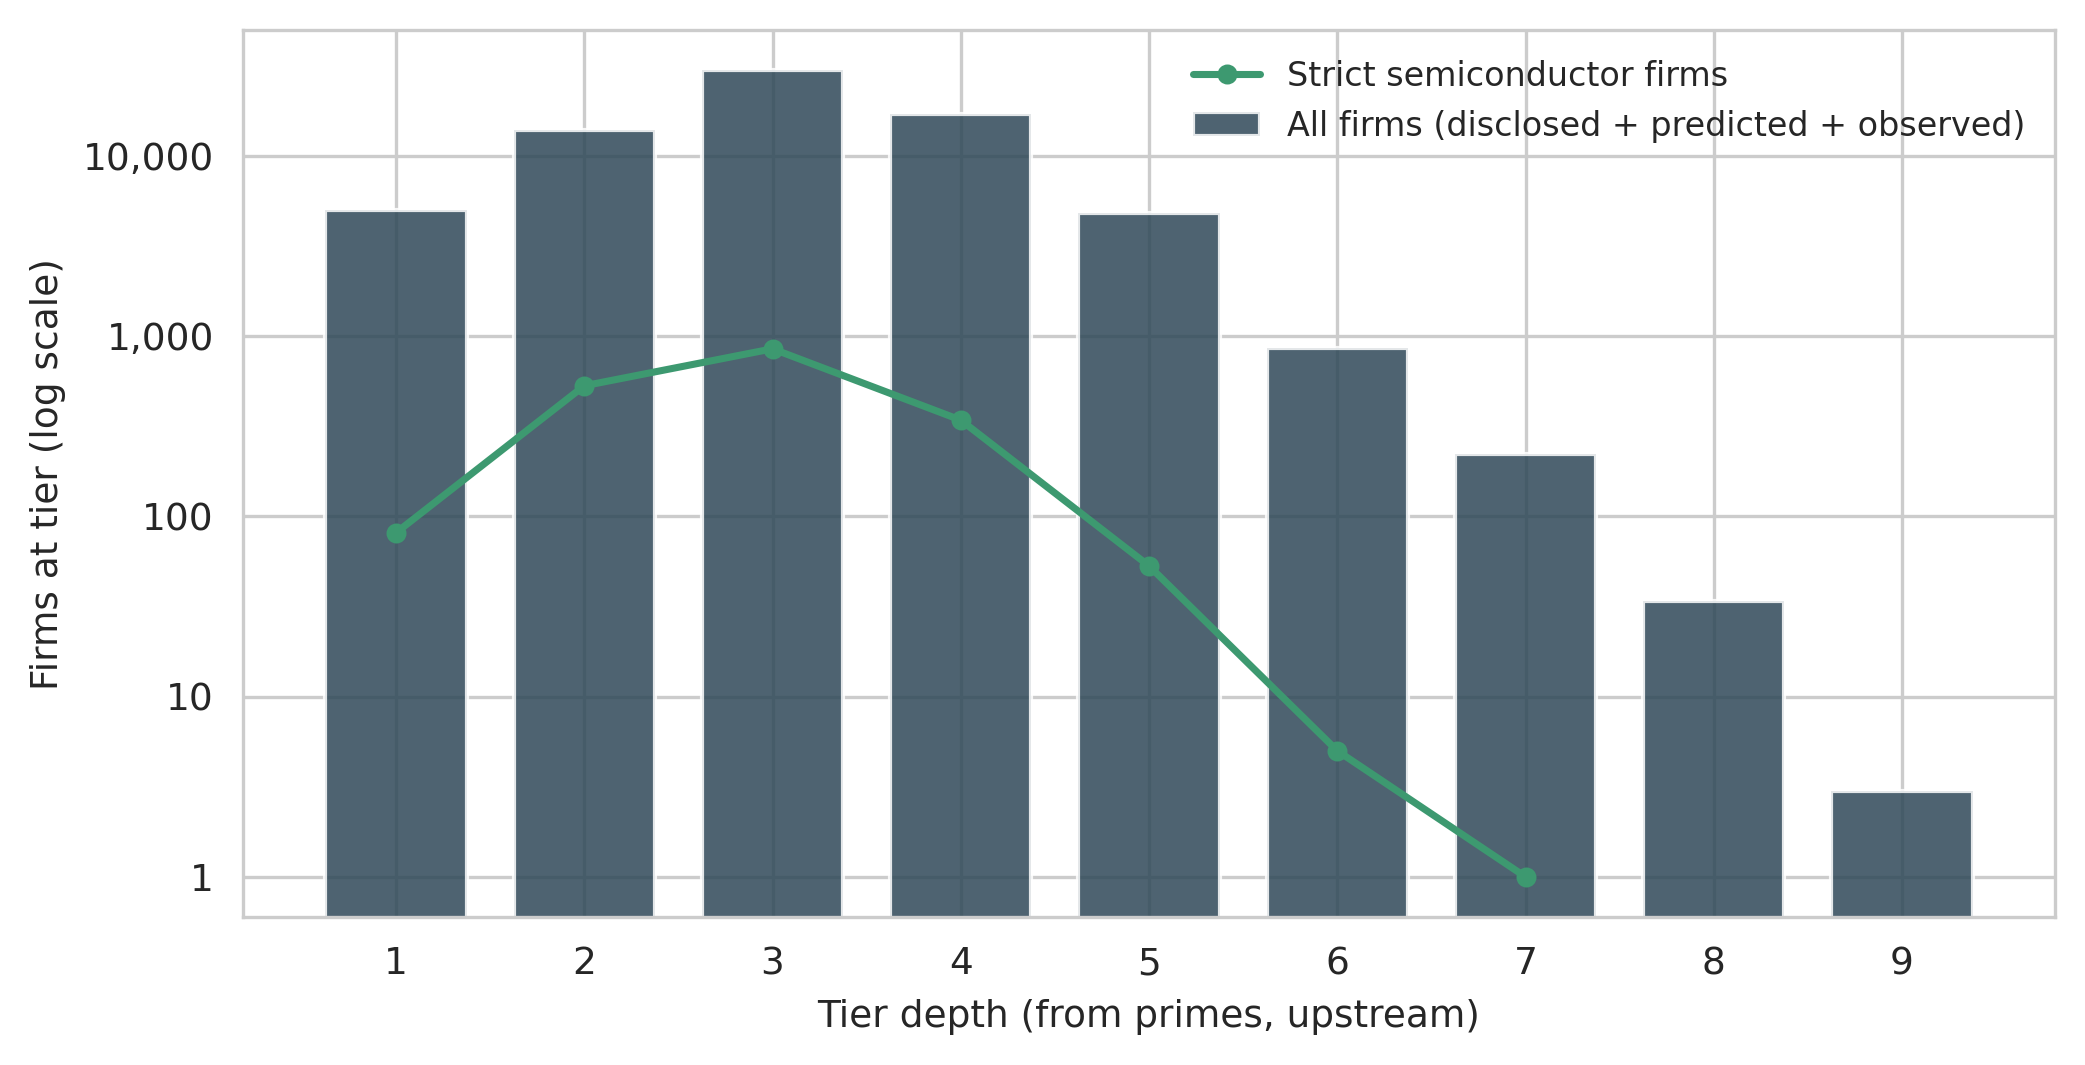
\includegraphics[width=\linewidth]{report/figures/fig_3.1_tier_depth_profile.png}

    \captionsetup{justification=raggedright,singlelinecheck=false}
    \caption*{\footnotesize \textit{Note}.  This figure summarizes the extent to which the locked DoD semiconductor network extends upstream from DoD prime contractors. The horizontal axis reports tier depth measured from Tier-1 primes: Tier 2 denotes firms that supply primes directly, Tier 3 denotes suppliers of those suppliers, and so on. Counts are computed over the commercial portion of the network using supply-like edges (disclosed SCR ties, Top-5 predicted supplier links, and observed shipper$\rightarrow$consignee shipping edges). Identity-bridge edges used to map prime contractor identities into the commercial firm universe are treated as stitching links for seeding and are not counted as supply ties. Bars show the total number of firms observed at each tier (log-scaled), and the line shows the subset of firms flagged as strict semiconductor firms under the RBICS L4 and/or SIC 3674 rule. The rapid expansion between tiers 2--4 and the long but thinning tail beyond tier 5 illustrates both the fan-out of disclosed/augmented supply dependencies around DoD-facing primes and the upstream placement of semiconductor-relevant activity within that dependency structure.}
\end{figure}

The depth profile in Figure~\ref{fig:tier-depth} is a compact check that the network is genuinely multi-tier rather than a one-hop supplier list. The rapid build-out in the first few tiers indicates that DoD-facing primes lie within a dense upstream neighborhood when the disclosed, predicted, and observed evidence is combined. In contrast, the thinning tail shows that upstream dependence continues beyond the near-prime layers. The strict semiconductor subset, primarily in the early tiers, reinforces that semiconductor-relevant activity is embedded within the near-prime dependency structure analyzed in Section~\ref{chap:network_analysis}, but is not confined to a single "chip-maker" layer.
Table~\ref{tab:ch3_evidence_overlap_deltas} provides a focused accounting of how the three supply-like evidence layers contribute unique directed firm pairs in the locked network. The ``incremental dyads'' block starts from the 251{,}054 disclosed supplier$\rightarrow$customer dyads and then adds 23{,}262 predicted dyads that are new relative to disclosure, yielding 274{,}316 dyads in the disclosed$\cup$predicted union. Adding observed shipping evidence then contributes 45{,}687 additional dyads that are new relative to that union, bringing the full disclosed$\cup$predicted$\cup$observed supply-like set to 320{,}003 directed dyads. The ``evidence overlap'' block reports the same 320{,}003 dyads partitioned into mutually exclusive categories, where most ties are supported by a single stream and a smaller share are supported by more than one. In this build, 249{,}935 dyads are disclosed only, 23{,}249 are predicted only, and 45{,}687 are observed only, while 1{,}119 dyads carry both disclosed and observed evidence, and 13 carry both predicted and observed evidence. There is no disclosed$\cap$predicted overlap, and no three-way overlap. Overlap is defined on the ordered pair, so direction matters. A shipping dyad overlaps a supply dyad only when the shipper$\rightarrow$consignee direction matches the supplier$\rightarrow$customer direction for the same two firms. This is why the observed layer's 46{,}819 shipping dyads translate into 45{,}687 incremental additions and \ShippingOverlap overlaps, and why evidence counts are not additive even though edge storage remains deduplicated by directed dyad.

% ---------- Evidence Overlap and Incremental Deltas ----------
\begin{table}[tbp]
\centering
\caption[\textit{Overlap and incremental deltas}]
{\textit{Overlap and Incremental Deltas in the DoD Semiconductor Network}}
\label{tab:ch3_evidence_overlap_deltas}

\begin{adjustbox}{max width=\linewidth}
\begin{tabular}{@{}l S[table-format=6.0, table-number-alignment=center]@{}}
\toprule
\multicolumn{1}{c}{Metric} & \multicolumn{1}{c}{Count} \\
\midrule
\multicolumn{2}{@{}l}{\textit{Incremental supply-edge dyads (directed)}} \\
Disclosed (as-of) & 251054 \\
+ Predicted (new vs disclosed) & 23262 \\
Disclosed $\cup$ predicted & 274316 \\
+ Observed (new vs disclosed$\cup$predicted) & 45687 \\
Disclosed $\cup$ predicted $\cup$ observed & 320003 \\
\midrule
\multicolumn{2}{@{}l}{\textit{Evidence overlap (mutually exclusive dyad categories)}} \\
Disclosed only & 249935 \\
Predicted only & 23249 \\
Observed only & 45687 \\
Disclosed $\cap$ Observed & 1119 \\
Predicted $\cap$ Observed & 13 \\
Disclosed $\cap$ Predicted & 0 \\
$\text{Disclosed} \cap \text{Predicted} \cap \text{Observed}$ & 0 \\
\bottomrule
\end{tabular}
\end{adjustbox}

\captionsetup{justification=raggedright,singlelinecheck=false}
\caption*{\footnotesize \textit{Note}. This table decomposes the \emph{supply-like} edge set in the DoD semiconductor network into disclosed SCR ties (as of the snapshot date), Top-$K$ predicted supplier links (Top-5 primary), and observed shipper$\rightarrow$consignee shipping edges. \emph{Incremental dyads} reports the number of \emph{unique directed firm pairs} admitted under (i) disclosed only, (ii) disclosed$\cup$predicted, and (iii) disclosed$\cup$predicted$\cup$observed, where overlaps are deduplicated by ordered pair. The \emph{Evidence overlap} block partitions the same directed dyads into mutually exclusive categories (single-evidence vs multi-evidence). Overlapping dyads are stored once in the multiplex with multiple evidence indicators, so overlaps increase provenance richness rather than inflating edge counts.}%
\end{table}

A relatively thin overlap across streams is not a weakness of the build. It is a predictable consequence of combining evidence regimes that are biased in different directions and therefore illuminate different parts of the same dependency structure. Disclosed SCR ties are shaped by what large, disclosure-intensive firms reveal through public reporting and related materials, which tends to emphasize stable, material relationships and counterparties that are themselves visible in the public corporate record. The predicted layer is constructed to push in the opposite direction. It is explicitly designed to recover relationships that are plausibly present but not disclosed, especially in the semiconductor-relevant portion of the graph, where non-observation is most consequential. The observed shipping layer is different again. It captures transaction evidence generated by cross-border logistics and bill-of-lading reporting, which can reveal counterparties that are not disclosure-intensive and may lie outside the set of firms that consistently appear in corporate supply-chain narratives. Overlap is useful as corroboration when it occurs, but the main value of the accounting in Table~\ref{tab:ch3_evidence_overlap_deltas} is that it shows the layers are largely complementary. Together, they expand coverage beyond what any single stream would reveal, while preserving provenance, so that Section~\ref{chap:network_analysis} can condition results on the evidence type rather than treating the merged network as a single undifferentiated source.

Taken together, Table~\ref{tab:ch3_dod_semiconductor_network_summary}, Figure~\ref{fig:tier-depth}, and Table~\ref{tab:ch3_evidence_overlap_deltas} describe the locked object that Section~\ref{chap:network_analysis} treats as fixed. The network is sufficiently large to capture multi-tier dependencies among DoD-facing primes. Still, it remains disciplined by a strict semiconductor boundary and a point-in-time build, which keeps evidence streams comparable. Just as importantly, provenance remains explicit at the dyad level. This makes it possible to report results on the full multiplex while also running sensitivity checks that condition on evidence type, such as disclosed-only, disclosed plus predicted, or the full disclosed plus predicted plus observed view, without changing the underlying definition of the DoD-anchored semiconductor scope established in \S3.6. The remaining visibility limits that persist even after layering and pruning clarify how those limits condition the interpretation of Section~\ref{chap:network_analysis}'s analytical results.

%========================
% Section 3.8
%========================
\section{Limitations and Summary}

Section~\ref{sec:descriptive-summary} provides an accounting of what the DoD semiconductor network contains and how the disclosed, predicted, and observed layers contribute to coverage (Table~\ref{tab:ch3_dod_semiconductor_network_summary}; Table~\ref{tab:ch3_evidence_overlap_deltas}). The discussion states the main limits of visibility that remain even after layering and pruning, and explains how those limits condition the interpretation of Section~\ref{chap:network_analysis}'s analytical results without previewing findings. Some of these limits are measurement error, including missingness in the underlying evidence streams and imperfect mapping across identifier systems that can prevent true dependencies from appearing in the constructed network. Others are scope choices the analysis explicitly makes, most importantly, the strict semiconductor boundary and the upstream retention rule defined in \S3.6, which shape which parts of the broader DoD-anchored multiplex are carried forward for analysis. The discussion is organized around the roles of the demand anchor, the three streams of relationship evidence, and the boundary and representation decisions that define the DoD semiconductor network. The central takeaway is that Section~\ref{chap:network_analysis} analyzes a defensible, provenance-aware snapshot of DoD-relevant semiconductor dependency structure, not a complete census, and the distinction matters for how absence, sparsity, and cross-layer disagreement should be interpreted.

The first visibility limit occurs when the network is anchored to DoD demand. USAspending links awarding components to prime recipients, but it does not provide systematic, transaction-grain visibility into subcontractors and lower-tier producers, which is where many semiconductor-relevant dependencies reside \parencite{U.S.GovernmentAccountabilityOffice2025}. Even when a prime is clearly connected to semiconductor activity downstream, the contracting tie itself should be read as an observed obligation relationship, not as evidence that the prime manufactures the relevant hardware or that the award maps cleanly onto a specific production chain (as discussed in \S3.1 and encoded as a distinct edge family in \S3.5). The contracting system also records administrative recipient identities that are optimized for reporting and legal accountability rather than for representing economic firm structure, so the demand anchor can overstate fragmentation across subsidiaries while understating consolidation at the corporate-family level. Finally, the anchor is tied to a recent but bounded reporting window under the snapshot discipline used here, so it captures a point-in-time view of which primes are visible to DoD procurement channels during that period rather than a full history of defense sourcing relationships. In Section~\ref{chap:network_analysis}, this means structural results should be interpreted as properties of the dependency network reachable from the observed prime-award anchor under these constraints, not as claims about the complete set of firms that contribute to defense-relevant semiconductor supply.

A second visibility limit comes from attrition in the identity linkage that connects Tier-1 primes to the commercial identifier spaces used for the relationship layers. First, some prime recipient identities in USAspending do not match any FactSet entity under the precision-first linkage policy, so they cannot serve as entry points for disclosed SCR ties, predicted links, or shipping-based observations. In this build, 43{,}794 of 71{,}967 primes link to FactSet entities, while 28{,}173 remain unmatched, and the matched set covers 75.3\% of total obligations, which implies that unmatched primes are disproportionately concentrated in the long tail by dollars. Second, even among primes that match FactSet entities, only a subset can be included in the SCR node universe, as this universe is required to attach disclosed SCR relationships and to receive SCR-based predicted supplier links. Concretely, 6{,}351 matched prime identities map into SCR and collapse to \NumPrimes unique SCR prime firm nodes. In contrast, the remaining FactSet-matched primes can still be connected through the contract anchor and, where available, shipping evidence, but cannot receive disclosed SCR traversal or predicted suppliers. In Section~\ref{chap:network_analysis}, these mechanisms imply that coverage differs systematically across evidence streams, so differences in apparent upstream structure across primes should be interpreted as provenance-conditioned visibility rather than as definitive evidence that some primes are truly isolated.

The disclosed layer inherits the core visibility limits of SCR as a disclosure-based relationship product. SCR coverage is incomplete and uneven across firm types, sectors, and geographies, so the absence of a disclosed supplier--customer tie is non-observation rather than evidence that no relationship exists (as emphasized in \S3.2). Disclosed relationships also reflect how firms describe and aggregate their counterparties in public materials, which can compress complex multi-entity supply arrangements into a single reported link and can leave some economically relevant counterparties outside the recorded graph. Timing adds a constraint because relationship start and end information is imperfect and subject to reporting lags, so an as-of snapshot can miss emerging ties and can retain ties that persist in disclosure even when operational dependence has shifted. Directionality should also be understood as a convention that makes the data usable for dependency analysis, since disclosed SCR ties are interpreted as supplier$\rightarrow$customer links, ensuring that upstream movement is well-defined. Still, the underlying disclosures are not generated for network inference. For Section~\ref{chap:network_analysis}, the implication is that any disclosed-only view is best interpreted as a conservative scaffold that is informative where it exists but should not be treated as a null claim about the absence of upstream dependence where it does not.

The predicted layer addresses one type of missingness, but it imposes its own explicit constraints. Predicted suppliers are generated only for Tier-1 primes that can be represented in the SCR node universe, and inference is limited to prime-adjacent supplier$\rightarrow$prime ties rather than attempting to populate deeper tiers by prediction (\S3.3). Candidate generation is itself a coverage limit, since only supplier--prime pairs that enter the bounded candidate pool are scored, and any omitted pairs are unscored and therefore unselectable under Top-$K$. Because the setting is positive--unlabeled, both false negatives and false positives are unavoidable, so predicted edges should be read as ranked evidence that expands visibility, not as confirmed relationships. A key deployment limitation is that the ensemble score is used in ranking mode rather than probability mode. In the construction setting, evaluation-time indicators used by the Section~\ref{chap:link-prediction} meta-ranker are unavailable and set to zero, so selection is implemented as a per-prime Top-$K$ rule without a probability floor (\S3.3). In Section~\ref{chap:network_analysis}, predicted ties are treated as provenance-tagged candidates, and their contribution is evaluated using sensitivity views, so scores are not interpreted as calibrated probabilities of a true supplier relationship.

The observed shipping layer provides event-level evidence, but it does not fully capture the semantics of dependence. A directed shipper$\rightarrow$consignee tie indicates that at least one shipment event was recorded within the inclusion window after cleaning and parent rollup, but it does not, on its own, establish a standing supplier relationship, contract duration, or input criticality (\S3.4). Coverage is also systematically uneven. Customs and bill-of-lading reporting shape the shipping feed and therefore tend to emphasize cross-border logistics, while domestic movements and non-maritime modalities are less consistently observed \parencite{factset_factset_2025}. The operational time index in this section is the dataset's record date, defined as the date the originating source distributed the record, not the underlying shipment date, so ``in-window'' should be read in that record-distribution sense (\S3.4). Even when parent rollups improve entity alignment, role labels can still reflect intermediated logistics, since freight forwarders, brokers, and traders can appear as shippers or consignees in ways that do not map cleanly onto supplier contracts. Entity concordance remains an additional constraint, since some counterparties are not linkable into the same identifier space as the disclosed supply graph, even when a shipment is observed. For Section~\ref{chap:network_analysis}, the practical implication is that observed ties are best interpreted as complementary adjacency and occasional corroboration of other evidence, rather than as a direct substitute for supplier--customer contracts or as a comprehensive census of material flows.

Finally, the DoD semiconductor network reflects explicit scope and representation decisions that shape what Section~\ref{chap:network_analysis} can claim. The boundary rule in \S3.6 retains three components: nodes and edges that lie on at least one directed semiconductor$\rightarrow$prime dependency path; the one-hop upstream suppliers of strict semiconductor firms; and, for deeper upstream structure, only when an upstream firm supplies at least two distinct semiconductor firms, which focuses attention on shared inputs. This rule is conservative by design, but it can exclude true dependencies that fall outside the strict semiconductor classification or that connect through pathways not observable under the section's evidence streams, especially for diversified firms whose semiconductor activity is difficult to classify cleanly (Appendix~\ref{app:semiconductor_classification_codes}). Representation also matters. The multiplex stores binary directed dyads rather than quantities, prices, or part-level provenance, and the same dyad can carry different meanings depending on whether it is supported by disclosure, prediction, or shipping evidence (\S3.5). Identity bridges stitch contracting identities to firm identifiers, allowing the demand anchor to attach to the commercial layers. Still, they are not dependency edges and should not be interpreted as economic relationships. In Section~\ref{chap:network_analysis}, these choices imply that results should be read as structure over a provenance-labeled approximation of dependence, suitable for comparative and robustness analysis across evidence types, but not as a weighted bill of materials or a platform-specific provenance trace.

In sum, Section~\ref{chap:dod-supply-chain} constructs a DoD-anchored semiconductor network that makes multi-tier dependence visible under a disciplined snapshot, while keeping the source of each relationship explicit. Starting from observed Tier-0$\rightarrow$Tier-1 procurement ties, the construction attaches disclosed supplier relationships, adds a high-confidence set of inferred prime-adjacent suppliers, and incorporates shipping-based observations, then restricts the result to a semiconductor-relevant subgraph using the strict boundary rule defined in \S3.6. The descriptive diagnostics in \S3.7 show that these evidence streams are largely complementary and that the resulting network is genuinely multi-tier, while also clarifying why coverage differs across primes and layers (Table~\ref{tab:ch3_evidence_overlap_deltas}). The limitations in this section imply that Section~\ref{chap:network_analysis} should interpret structure in provenance-aware terms, distinguishing what is visible by disclosure, what is suggested by prediction, and what is observed in shipment events, rather than treating the merged network as a single undifferentiated source. With those constraints in view, the network remains defensible as the report's empirical foundation because it is transparent about what it includes, reproducible under a fixed build, and explicit about what it cannot observe. Section~\ref{chap:network_analysis} takes this constructed object as fixed and uses it to characterize DoD-relevant semiconductor dependency structure under evidence-conditioned sensitivity views, without re-opening construction choices or treating any single layer as complete.

